\documentclass[a4paper,12pt,twoside]{article}

\usepackage[utf8]{inputenc}
\usepackage[T2A]{fontenc}
\usepackage[english]{babel}
\usepackage{booktabs}
\usepackage[margin = 1in]{geometry}
\usepackage{graphicx}
\usepackage{amsmath}
\usepackage{amssymb}
\usepackage{tikz}
\usepackage{fancyhdr}
\usepackage{subcaption}

\parindent=0pt
\parskip=10pt

\pagestyle{fancy}
\fancyhf{}
\rhead{sasha petrov}
\lhead{}
\rfoot{\thepage}

%hyperlinks package -- should be the last to import
\usepackage{hyperref}
\hypersetup{
	colorlinks = true,
	linkcolor=blue,
	citecolor=blue,
	urlcolor=blue }
	
\title{ECON 31703: Assignment 3}
\author{sasha petrov}

\begin{document}

\maketitle

\section*{(e)}

\begin{figure}[ht]
        \begin{minipage}[t]{0.45\linewidth}
            \centering
            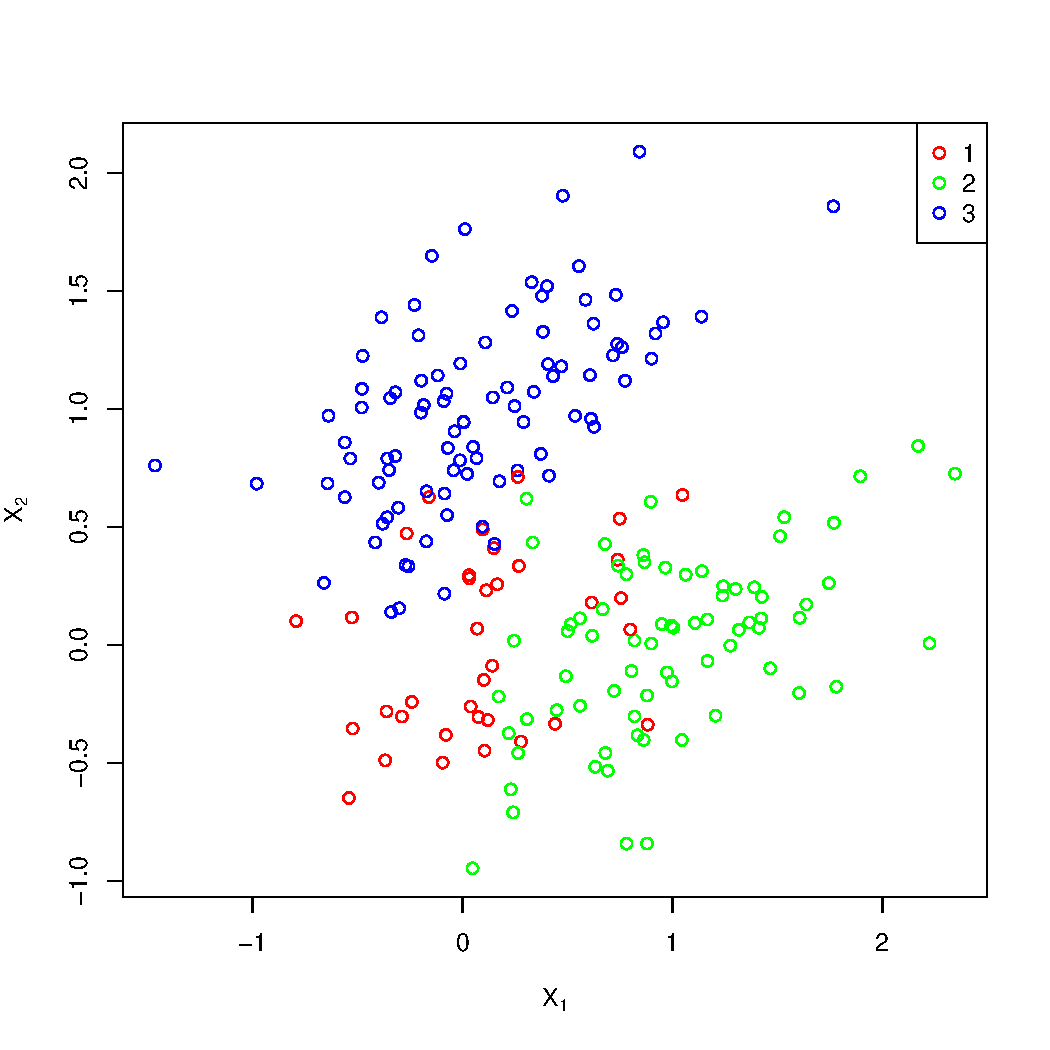
\includegraphics[width = \textwidth, keepaspectratio]{true_clustering.pdf}
                       \caption{true clustering}
            \label{fig:a}
        \end{minipage}
        \hspace{0.5cm}
        \begin{minipage}[t]{0.45\linewidth}
            \centering
            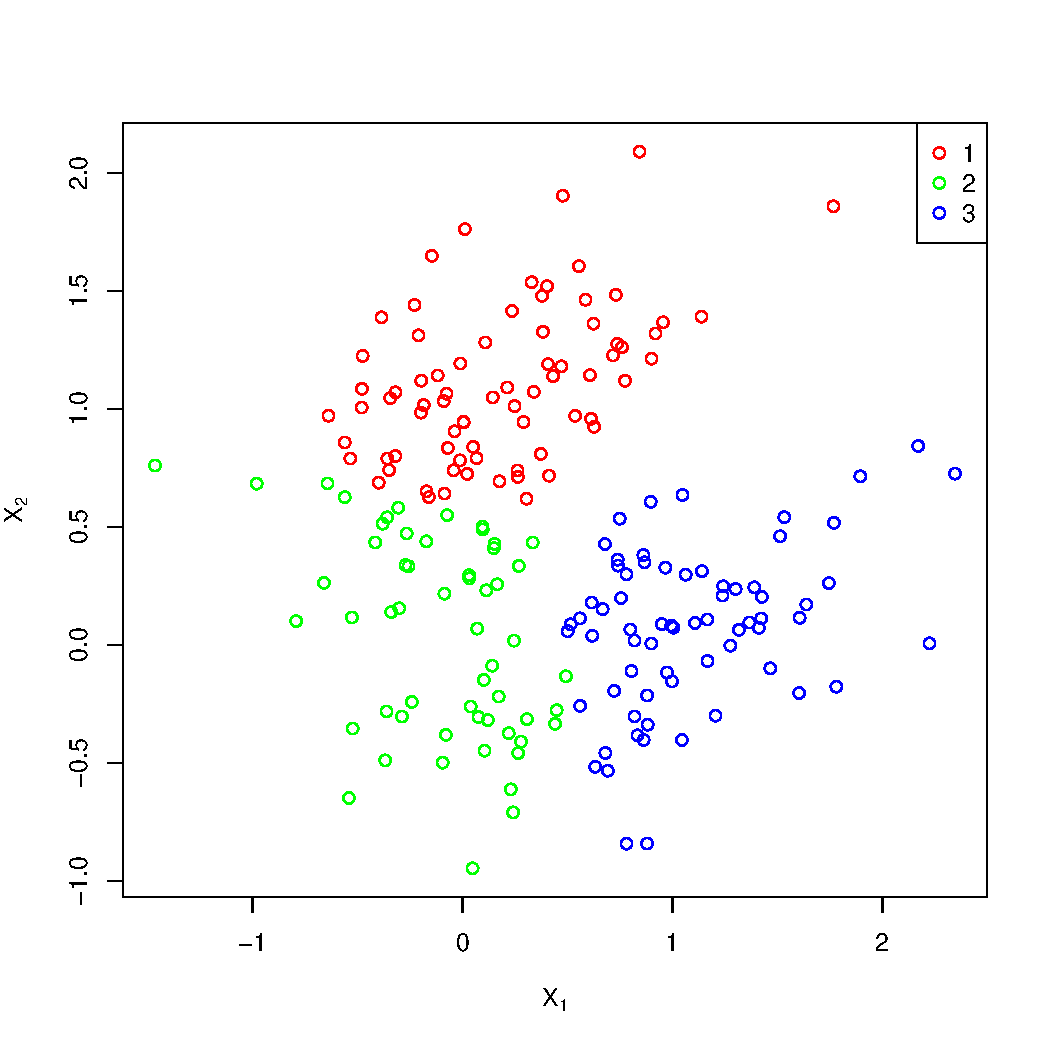
\includegraphics[width = \textwidth, keepaspectratio]{best_k_means.pdf}
                        \caption{best $k$-means}
            \label{fig:b}
        \end{minipage}
\end{figure}

Figure \ref{fig:b} captures the best partitioning of $X_i$-space into 3 clusters. Overall, it does a fair job of revealing the true hierarchical model (that is highlighted in figure \ref{fig:a}). However, importantly,  $k$-means fails to reflect a) the possibility of `overlap' among domains of models corresponding to different hyper-parameters; b) the difference in `weights' of different models. That is, $k$-means partitions the given `cloud' of data points into $3$ roughly equally-sized and non-intersecting sections on the plane.

Factors that seem important to me for how well $k$-means works:

\begin{itemize}
  \item distance between means of different hyper-models
	\begin{itemize}
	  \item in our case, it seems that distances are large enough to separate $3$ distinct areas
	\end{itemize}
  \item variance within each of the hyper-models
	\begin{itemize}
	  \item in our case, variances are quite low, which makes the risk of `overlapping' quite low and, thus, leads $k$-means to do a good job
	\end{itemize}
  \item correlation structure between covariates; shapes of `clouds' corresponding to different hyper-models matter: given the same variance, if there's higher correlation we expect less risk of `overlapping' (intuitively, ellipsoids that are prolongated in the same direction are harder to intersect than circles)
	\begin{itemize}
	  \item in our case, there is some positive correlation between $X_1$ and $X_2$, which probably helps the algorithm to avoid building clusters that have a `wrong' shape
	\end{itemize}
\end{itemize}


\section*{(f)}

\begin{table}[h]
\centering
\caption{trying different \( \tilde K \)}
\label{tab:k_tilde}
\begin{tabular}{lcccc}
\toprule
\( \tilde K \) & 2 & 3 & 4 & 5 \\ 
  \midrule
bias & 0.47 & 0.18 & 0.07 & 0.04 \\ 
variance & 0.01 & 0.02 & 0.03 & 0.03 \\ 
\bottomrule
\end{tabular}
\end{table}

Table \ref{tab:k_tilde} reports average biases and variances (as defined in the problem set) for \( 4 \) different values of $\tilde K$. We see something that resembles a classic bias-variance trade-off. As the number of suggested clusters increases, the average bias goes down dramatically but at the cost of the increasing variance of estimates. Interestingly, the shifts along this trade-off become less pronounced as the number of clusters increases. The reason for this is probably that once the number of clusters becomes sufficiently high, some of them are negligibly different (because they capture points from the same hyper-model); therefore, we shouldn't expect to see a change in patterns of $ \mu_{\theta_i 1}$ across some subsets of clusters; in other words, both $\bar \mu_{k_i} - \mu_{\theta_i 1}$ and $Y_i - \mu_{\theta_i 1}$ won't change much when we `split' certain clusters.


\end{document}